\documentclass[11pt, oneside]{article}   	% use "amsart" instead of "article" for AMSLaTeX format
\usepackage{geometry}                		
\usepackage{blindtext}
\usepackage[utf8]{inputenc}
\usepackage[greek,english]{babel}
\usepackage{alphabeta}
\geometry{letterpaper}                   		% ... or a4paper or a5paper or ... 
%\geometry{landscape}                		% Activate for rotated page geometry
%\usepackage[parfill]{parskip}    		% Activate to begin paragraphs with an empty line rather than an indent
\usepackage{graphicx}				% Use pdf, png, jpg, or eps§ with pdflatex; use eps in DVI mode
								% TeX will automatically convert eps --> pdf in pdflatex		
\usepackage{amssymb}
\usepackage{tikz}
\usetikzlibrary{angles, quotes}
\usepackage{booktabs} % For better table formatting
\usepackage{xcolor}

%SetFonts

%SetFonts


\title{Εργασία Υπολογιστικής Γεωμετρίας}
\author{Κωνσταντίνος Ζουριδάκης 1115202000254}
\date{}							% Activate to display a given date or no date

\begin{document}


\maketitle

\newpage
\tableofcontents
\newpage

\section{Υλοποίηση Α: Κυρτό περίβλημα}
\subsection{Υλοποίηση αλγορίθμων}

\begin{center}
 \Large \textbf{Αυξητικός Αλγόριθμος} 
 \end{center}

Το παράδειγμα που υλοποιώ στον κώδικά μου για τον αυξητικό αλγόριθμο εμφανίζεται παρακάτω με ενωμένα τα σημεία του αποτελέσματος τα οποία αποτελούν το κυρτό περίβλημα.

\centering
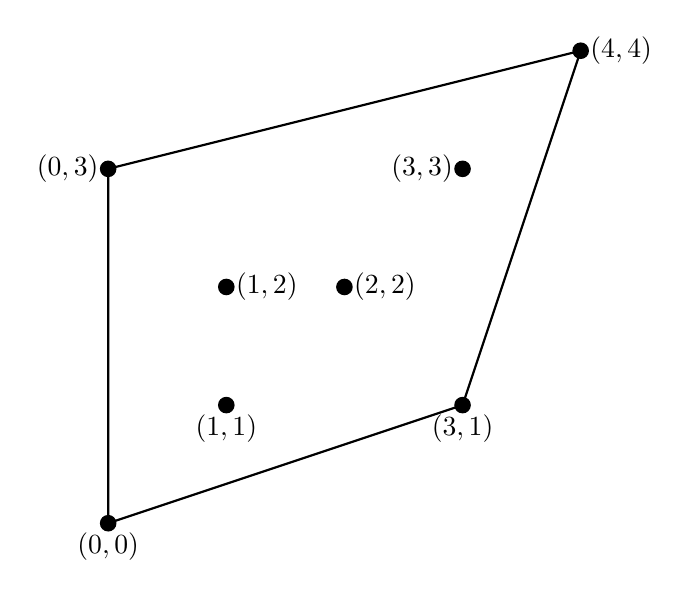
\begin{tikzpicture}[scale=1.5]

    % Points
    \coordinate (P1) at (0, 3);
    \coordinate (P2) at (1, 1);
    \coordinate (P3) at (2, 2);
    \coordinate (P4) at (4, 4);
    \coordinate (P5) at (0, 0);
    \coordinate (P6) at (1, 2);
    \coordinate (P7) at (3, 1);
    \coordinate (P8) at (3, 3);
    
    % Draw points
    \foreach \p/\x in {(P1), (P2), (P3), (P4), (P5), (P6), (P7), (P8)} {
        \fill \p circle (2pt);
    }

    % Label points
    \node[anchor=east] at (P1) {$(0,3)$};
    \node[anchor=north] at (P2) {$(1,1)$};
    \node[anchor=west] at (P3) {$(2,2)$};
    \node[anchor=west] at (P4) {$(4,4)$};
    \node[anchor=north] at (P5) {$(0,0)$};
    \node[anchor=west] at (P6) {$(1,2)$};
    \node[anchor=north] at (P7) {$(3,1)$};
    \node[anchor=east] at (P8) {$(3,3)$};

    % Convex hull (using Graham's scan result)
    \draw[thick] (P5) -- (P1) -- (P4) -- (P7) -- (P5) -- cycle;


\end{tikzpicture}

\newpage

Τα βήματα που ακολουθεί ο αλγόριθμος εμφανίζεται γραφικά παρακάτω:

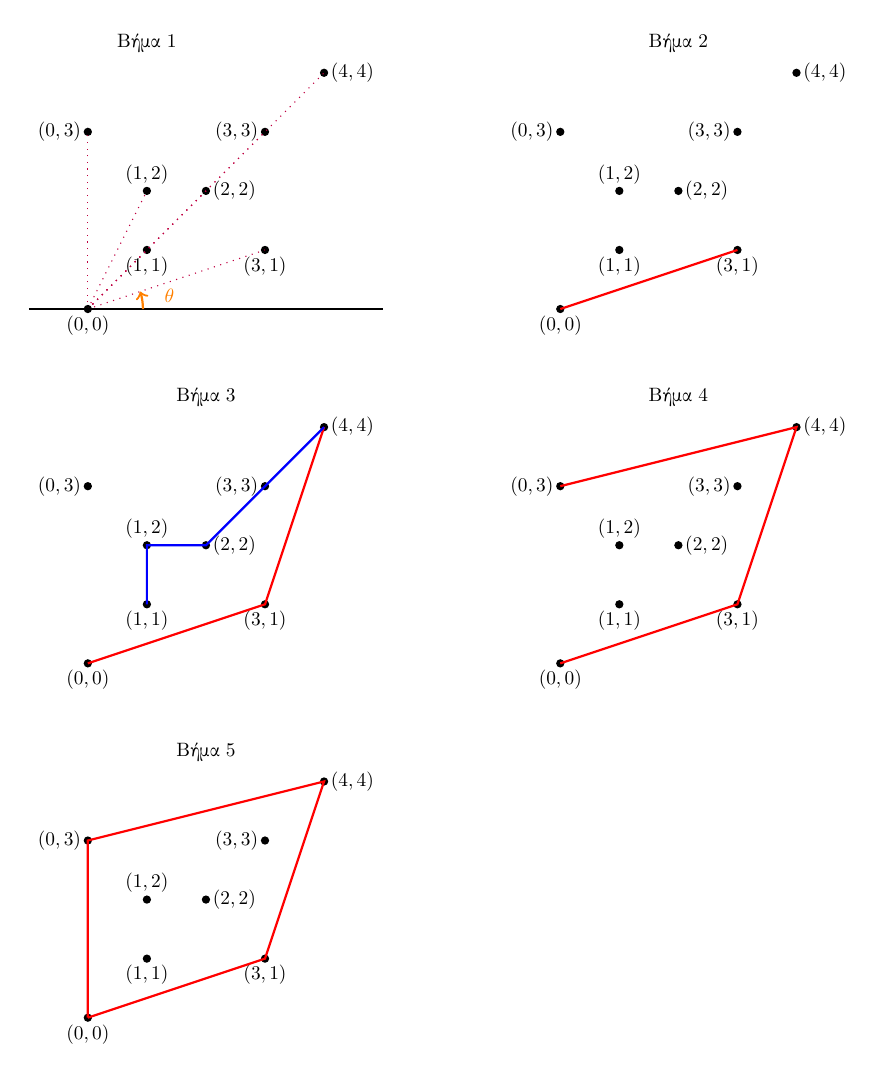
\begin{tikzpicture}[scale=0.75, every node/.style={scale=0.7}]

    % Step 1: Plot all points
    \begin{scope}[shift={(0, 0)}]
        \node at (1, 4.5) {Βήμα 1};
        \coordinate (P1) at (0, 3);
        \coordinate (P2) at (1, 1);
        \coordinate (P3) at (2, 2);
        \coordinate (P4) at (4, 4);
        \coordinate (P5) at (0, 0);
        \coordinate (P6) at (1, 2);
        \coordinate (P7) at (3, 1);
        \coordinate (P8) at (3, 3);
        \coordinate (P9) at (1,0);

        % Draw points
        \foreach \p/\x in {(P1), (P2), (P3), (P4), (P5), (P6), (P7), (P8)} {
            \fill \p circle (2pt);
        }
        \draw[dotted, purple] (0,0) -- (3,1);
        \draw[dotted, purple] (0,0) -- (1,1);
        \draw[dotted, purple] (0,0) -- (3,3);
        \draw[dotted, purple] (0,0) -- (2,2);
        \draw[dotted, purple] (0,0) -- (1,2);
        \draw[dotted, purple] (0,0) -- (4,4);
        \draw[dotted, purple] (0,0) -- (0,3);
        \draw[thick] (-1,0) -- (5,0);
        \pic [draw, ->,"$\theta$", orange, thick, angle radius=1cm, angle eccentricity=1.5] {angle = P9--P5--P7};

        % Label points
        \node[anchor=east] at (P1) {$(0,3)$};
        \node[anchor=north] at (P2) {$(1,1)$};
        \node[anchor=west] at (P3) {$(2,2)$};
        \node[anchor=west] at (P4) {$(4,4)$};
        \node[anchor=north] at (P5) {$(0,0)$};
        \node[anchor=south] at (P6) {$(1,2)$};
        \node[anchor=north] at (P7) {$(3,1)$};
        \node[anchor=east] at (P8) {$(3,3)$};
    \end{scope}
    
    % Step 3: Start Lower Hull
    \begin{scope}[shift={(8, 0)}]
        \node at (2, 4.5) {Βήμα 2};
        % Draw points
        \fill (0, 0) circle (2pt) node[anchor=north] {$(0,0)$};
        \fill (1, 1) circle (2pt) node[anchor=north] {$(1,1)$};
        \fill (2, 2) circle (2pt) node[anchor=west] {$(2,2)$};
        \fill (3, 1) circle (2pt) node[anchor=north] {$(3,1)$};
        \fill (4, 4) circle (2pt) node[anchor=west] {$(4,4)$};
        \fill (0, 3) circle (2pt) node[anchor=east] {$(0,3)$};
        \fill (3, 3) circle (2pt) node[anchor=east] {$(3,3)$};
        \fill (1, 2) circle (2pt) node[anchor=south] {$(1,2)$};

        % Draw first edges of lower hull
        \draw[thick, red] (0,0) -- (3,1);
    \end{scope}
    
    
        % Step 3: Start Lower Hull
    \begin{scope}[shift={(0, -6)}]
        \node at (2, 4.5) {Βήμα 3};
        % Draw points
        \fill (0, 0) circle (2pt) node[anchor=north] {$(0,0)$};
        \fill (1, 1) circle (2pt) node[anchor=north] {$(1,1)$};
        \fill (2, 2) circle (2pt) node[anchor=west] {$(2,2)$};
        \fill (3, 1) circle (2pt) node[anchor=north] {$(3,1)$};
        \fill (4, 4) circle (2pt) node[anchor=west] {$(4,4)$};
        \fill (0, 3) circle (2pt) node[anchor=east] {$(0,3)$};
        \fill (3, 3) circle (2pt) node[anchor=east] {$(3,3)$};
        \fill (1, 2) circle (2pt) node[anchor=south] {$(1,2)$};

        % Draw first edges of lower hull
        \draw[thick, red] (0,0) -- (3,1) -- (4,4);
        \draw[thick, blue] (4,4) -- (3,3) -- (2,2) -- (1,2) -- (1,1);
    \end{scope}
    
    \begin{scope}[shift={(8, -6)}]
        \node at (2, 4.5) {Βήμα 4};
        % Draw points
        \fill (0, 0) circle (2pt) node[anchor=north] {$(0,0)$};
        \fill (1, 1) circle (2pt) node[anchor=north] {$(1,1)$};
        \fill (2, 2) circle (2pt) node[anchor=west] {$(2,2)$};
        \fill (3, 1) circle (2pt) node[anchor=north] {$(3,1)$};
        \fill (4, 4) circle (2pt) node[anchor=west] {$(4,4)$};
        \fill (0, 3) circle (2pt) node[anchor=east] {$(0,3)$};
        \fill (3, 3) circle (2pt) node[anchor=east] {$(3,3)$};
        \fill (1, 2) circle (2pt) node[anchor=south] {$(1,2)$};

        % Draw first edges of lower hull
        \draw[thick, red] (0,0) -- (3,1) -- (4,4) -- (0,3);
    \end{scope}
    
    \begin{scope}[shift={(0, -12)}]
        \node at (2, 4.5) {Βήμα 5};
        % Draw points
        \fill (0, 0) circle (2pt) node[anchor=north] {$(0,0)$};
        \fill (1, 1) circle (2pt) node[anchor=north] {$(1,1)$};
        \fill (2, 2) circle (2pt) node[anchor=west] {$(2,2)$};
        \fill (3, 1) circle (2pt) node[anchor=north] {$(3,1)$};
        \fill (4, 4) circle (2pt) node[anchor=west] {$(4,4)$};
        \fill (0, 3) circle (2pt) node[anchor=east] {$(0,3)$};
        \fill (3, 3) circle (2pt) node[anchor=east] {$(3,3)$};
        \fill (1, 2) circle (2pt) node[anchor=south] {$(1,2)$};

        % Draw first edges of lower hull
        \draw[thick, red] (0,0) -- (3,1) -- (4,4) -- (0,3) -- (0,0);
    \end{scope}
    
  
\end{tikzpicture}

\newpage

\begin{center} \Large \textbf{Αλγόριθμος του Περιτυλίγματος} \end{center}

Το παράδειγμα που υλοποιώ στον κώδικά μου για τον αλγόριθμο του περιτυλίγματος εμφανίζεται παρακάτω:

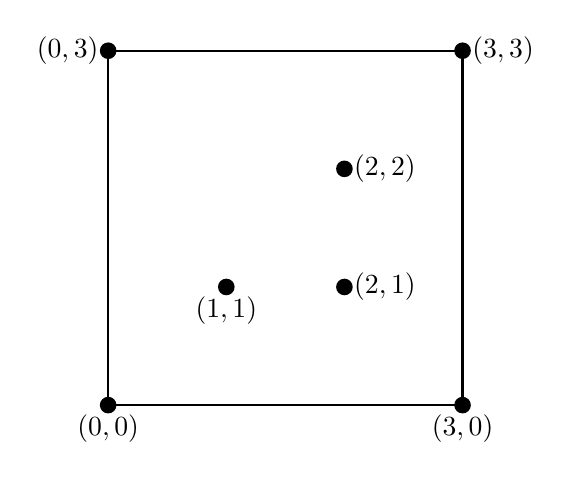
\begin{tikzpicture}[scale=1.5]

    % Coordinates for the points
    \coordinate (P1) at (0, 3);  % (0, 3)
    \coordinate (P2) at (2, 2);  % (2, 2)
    \coordinate (P3) at (1, 1);  % (1, 1)
    \coordinate (P4) at (2, 1);  % (2, 1)
    \coordinate (P5) at (3, 0);  % (3, 0)
    \coordinate (P6) at (0, 0);  % (0, 0)
    \coordinate (P7) at (3, 3);  % (3, 3)

    % Draw the points
    \fill (P1) circle (2pt) node[anchor=east] {$(0,3)$};
    \fill (P2) circle (2pt) node[anchor=west] {$(2,2)$};
    \fill (P3) circle (2pt) node[anchor=north] {$(1,1)$};
    \fill (P4) circle (2pt) node[anchor=west] {$(2,1)$};
    \fill (P5) circle (2pt) node[anchor=north] {$(3,0)$};
    \fill (P6) circle (2pt) node[anchor=north] {$(0,0)$};
    \fill (P7) circle (2pt) node[anchor=west] {$(3,3)$};

    % Draw the convex hull edges
    \draw[thick] (P6) -- (P5);  % (0,0) to (3,0)
    \draw[thick] (P5) -- (P7);  % (3,0) to (3,3)
    \draw[thick] (P7) -- (P1);  % (3,3) to (0,3)
    \draw[thick] (P1) -- (P6);  % (0,3) to (0,0)

\end{tikzpicture}

\newpage

Τα βήματα παρουσιάζονται γραφικά παρακάτω:

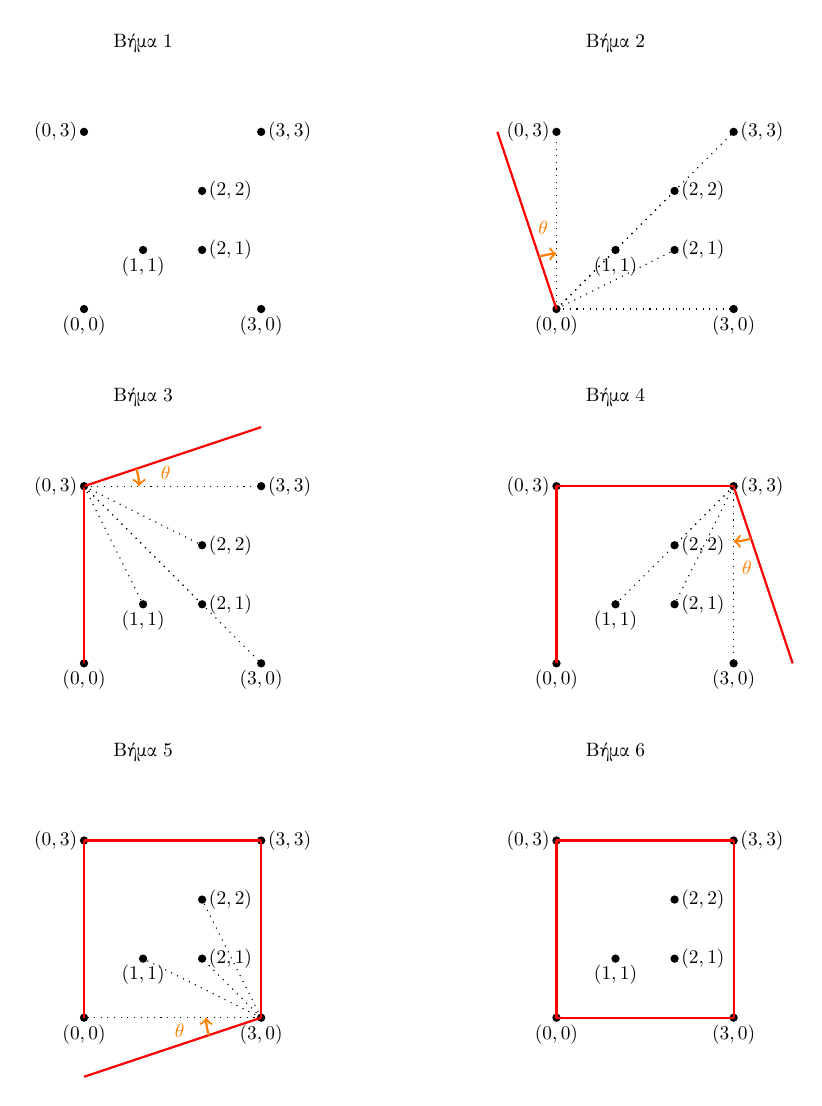
\begin{tikzpicture}[scale=0.75, every node/.style={scale=0.7}]

    % Step 1: Plot all points
    \begin{scope}[shift={(0, 0)}]
        \node at (1, 4.5) {Βήμα 1};
        \coordinate (P1) at (0, 3);  % (0, 3)
    	\coordinate (P2) at (2, 2);  % (2, 2)
    	\coordinate (P3) at (1, 1);  % (1, 1)
    	\coordinate (P4) at (2, 1);  % (2, 1)
    	\coordinate (P5) at (3, 0);  % (3, 0)
    	\coordinate (P6) at (0, 0);  % (0, 0)
    	\coordinate (P7) at (3, 3);  % (3, 3)

        % Draw the points
    	\fill (P1) circle (2pt) node[anchor=east] {$(0,3)$};
    	\fill (P2) circle (2pt) node[anchor=west] {$(2,2)$};
    	\fill (P3) circle (2pt) node[anchor=north] {$(1,1)$};
    	\fill (P4) circle (2pt) node[anchor=west] {$(2,1)$};
    	\fill (P5) circle (2pt) node[anchor=north] {$(3,0)$};
    	\fill (P6) circle (2pt) node[anchor=north] {$(0,0)$};
    	\fill (P7) circle (2pt) node[anchor=west] {$(3,3)$};
    \end{scope}
    
    \begin{scope}[shift={(8, 0)}]
        \node at (1, 4.5) {Βήμα 2};
        \coordinate (P1) at (0, 3);  % (0, 3)
    	\coordinate (P2) at (2, 2);  % (2, 2)
    	\coordinate (P3) at (1, 1);  % (1, 1)
    	\coordinate (P4) at (2, 1);  % (2, 1)
    	\coordinate (P5) at (3, 0);  % (3, 0)
    	\coordinate (P6) at (0, 0);  % (0, 0)
    	\coordinate (P7) at (3, 3);  % (3, 3)
		\coordinate (P8) at (-1,3);
		\coordinate (P9) at (0,1.5);

        % Draw the points
    	\fill (P1) circle (2pt) node[anchor=east] {$(0,3)$};
    	\fill (P2) circle (2pt) node[anchor=west] {$(2,2)$};
    	\fill (P3) circle (2pt) node[anchor=north] {$(1,1)$};
    	\fill (P4) circle (2pt) node[anchor=west] {$(2,1)$};
    	\fill (P5) circle (2pt) node[anchor=north] {$(3,0)$};
    	\fill (P6) circle (2pt) node[anchor=north] {$(0,0)$};
    	\fill (P7) circle (2pt) node[anchor=west] {$(3,3)$};
	
		\draw[dotted] (P6) -- (P1);
		\draw[dotted] (P6) -- (P2);
		\draw[dotted] (P6) -- (P3);
		\draw[dotted] (P6) -- (P4);
		\draw[dotted] (P6) -- (P5);
		\draw[dotted] (P6) -- (P7);
		\draw[thick,red] (P6) -- (P8);
		\pic [draw, <-,"$\theta$", orange, thick, angle radius=1cm, angle eccentricity=1.5] {angle = P1--P6--P8};  % Measure the angle

		
    \end{scope}
    
    \begin{scope}[shift={(0, -6)}]
        \node at (1, 4.5) {Βήμα 3};
        \coordinate (P1) at (0, 3);  % (0, 3)
    	\coordinate (P2) at (2, 2);  % (2, 2)
    	\coordinate (P3) at (1, 1);  % (1, 1)
    	\coordinate (P4) at (2, 1);  % (2, 1)
    	\coordinate (P5) at (3, 0);  % (3, 0)
    	\coordinate (P6) at (0, 0);  % (0, 0)
    	\coordinate (P7) at (3, 3);  % (3, 3)
		\coordinate (P8) at (3, 4);

        % Draw the points
    	\fill (P1) circle (2pt) node[anchor=east] {$(0,3)$};
    	\fill (P2) circle (2pt) node[anchor=west] {$(2,2)$};
    	\fill (P3) circle (2pt) node[anchor=north] {$(1,1)$};
    	\fill (P4) circle (2pt) node[anchor=west] {$(2,1)$};
    	\fill (P5) circle (2pt) node[anchor=north] {$(3,0)$};
    	\fill (P6) circle (2pt) node[anchor=north] {$(0,0)$};
    	\fill (P7) circle (2pt) node[anchor=west] {$(3,3)$};
	
		\draw[thick, red] (P6) -- (P1);
		\draw [thick,red] (P1) -- (P8);
		\draw[dotted] (P1) -- (P2);
		\draw[dotted] (P1) -- (P3);
		\draw[dotted] (P1) -- (P4);
		\draw[dotted] (P1) -- (P5);
		\draw[dotted] (P1) -- (P7);
		\pic [draw, <-,"$\theta$", orange, thick, angle radius=1cm, angle eccentricity=1.5] {angle = P7--P1--P8};  % Measure the angle
    \end{scope}
    
    \begin{scope}[shift={(8, -6)}]
        \node at (1, 4.5) {Βήμα 4};
        \coordinate (P1) at (0, 3);  % (0, 3)
    	\coordinate (P2) at (2, 2);  % (2, 2)
    	\coordinate (P3) at (1, 1);  % (1, 1)
    	\coordinate (P4) at (2, 1);  % (2, 1)
    	\coordinate (P5) at (3, 0);  % (3, 0)
    	\coordinate (P6) at (0, 0);  % (0, 0)
    	\coordinate (P7) at (3, 3);  % (3, 3)
		\coordinate (P8) at (4, 0);

        % Draw the points
    	\fill (P1) circle (2pt) node[anchor=east] {$(0,3)$};
    	\fill (P2) circle (2pt) node[anchor=west] {$(2,2)$};
    	\fill (P3) circle (2pt) node[anchor=north] {$(1,1)$};
    	\fill (P4) circle (2pt) node[anchor=west] {$(2,1)$};
    	\fill (P5) circle (2pt) node[anchor=north] {$(3,0)$};
    	\fill (P6) circle (2pt) node[anchor=north] {$(0,0)$};
    	\fill (P7) circle (2pt) node[anchor=west] {$(3,3)$};
	
		\draw[thick, red] (P6) -- (P1);
		\draw[thick,red] (P7) -- (P8);
		\draw[dotted] (P7) -- (P2);
		\draw[dotted] (P7) -- (P3);
		\draw[dotted] (P7) -- (P4);
		\draw[dotted] (P7) -- (P5);
		\draw[thick, red] (P1) -- (P7);
		\pic [draw, <-,"$\theta$", orange, thick, angle radius=1cm, angle eccentricity=1.5] {angle = P5--P7--P8};  % Measure the angle
    \end{scope}
    
    \begin{scope}[shift={(0, -12)}]
        \node at (1, 4.5) {Βήμα 5};
        \coordinate (P1) at (0, 3);  % (0, 3)
    	\coordinate (P2) at (2, 2);  % (2, 2)
    	\coordinate (P3) at (1, 1);  % (1, 1)
    	\coordinate (P4) at (2, 1);  % (2, 1)
    	\coordinate (P5) at (3, 0);  % (3, 0)
    	\coordinate (P6) at (0, 0);  % (0, 0)
    	\coordinate (P7) at (3, 3);  % (3, 3)
		\coordinate (P8) at (0, -1);

        % Draw the points
    	\fill (P1) circle (2pt) node[anchor=east] {$(0,3)$};
    	\fill (P2) circle (2pt) node[anchor=west] {$(2,2)$};
    	\fill (P3) circle (2pt) node[anchor=north] {$(1,1)$};
    	\fill (P4) circle (2pt) node[anchor=west] {$(2,1)$};
    	\fill (P5) circle (2pt) node[anchor=north] {$(3,0)$};
    	\fill (P6) circle (2pt) node[anchor=north] {$(0,0)$};
    	\fill (P7) circle (2pt) node[anchor=west] {$(3,3)$};
	
		\draw[thick, red] (P6) -- (P1);
		\draw[thick,red] (P5) -- (P8);
		\draw[dotted] (P5) -- (P2);
		\draw[dotted] (P5) -- (P3);
		\draw[dotted] (P5) -- (P4);
		\draw[dotted] (P5) -- (P6);
		\draw[thick, red] (P7) -- (P5);
		\draw[thick, red] (P1) -- (P7);
		\pic [draw, <-,"$\theta$", orange, thick, angle radius=1cm, angle eccentricity=1.5] {angle = P6--P5--P8};  % Measure the angle
    \end{scope}
    
    \begin{scope}[shift={(8, -12)}]
        \node at (1, 4.5) {Βήμα 6};
        \coordinate (P1) at (0, 3);  % (0, 3)
    	\coordinate (P2) at (2, 2);  % (2, 2)
    	\coordinate (P3) at (1, 1);  % (1, 1)
    	\coordinate (P4) at (2, 1);  % (2, 1)
    	\coordinate (P5) at (3, 0);  % (3, 0)
    	\coordinate (P6) at (0, 0);  % (0, 0)
    	\coordinate (P7) at (3, 3);  % (3, 3)

        % Draw the points
    	\fill (P1) circle (2pt) node[anchor=east] {$(0,3)$};
    	\fill (P2) circle (2pt) node[anchor=west] {$(2,2)$};
    	\fill (P3) circle (2pt) node[anchor=north] {$(1,1)$};
    	\fill (P4) circle (2pt) node[anchor=west] {$(2,1)$};
    	\fill (P5) circle (2pt) node[anchor=north] {$(3,0)$};
    	\fill (P6) circle (2pt) node[anchor=north] {$(0,0)$};
    	\fill (P7) circle (2pt) node[anchor=west] {$(3,3)$};
	
		\draw[thick, red] (P6) -- (P1);
		\draw[thick,red] (P5) -- (P6);
		\draw[thick, red] (P7) -- (P5);
		\draw[thick, red] (P1) -- (P7);
    \end{scope}
    
      
\end{tikzpicture}

\newpage

\begin{center} \Large \textbf{Διαίρει και Βασίλευε} \end{center}

Το παράδειγμα το οποίο χρησιμοποιώ στον κώδικά μου είναι το παρακάτω:

\begin{tikzpicture}[scale=0.75]

    % Coordinates for the points
    \coordinate (P1) at (0, 0);    % (0, 0)
    \coordinate (P2) at (0, 4);    % (0, 4)
    \coordinate (P3) at (-4, 0);   % (-4, 0)
    \coordinate (P4) at (5, 0);    % (5, 0)
    \coordinate (P5) at (0, -6);   % (0, -6)
    \coordinate (P6) at (1, 0);    % (1, 0)

    % Draw the points
    \fill (P1) circle (3pt) node[anchor=north] {$(0, 0)$};
    \fill (P2) circle (3pt) node[anchor=west] {$(0, 4)$};
    \fill (P3) circle (3pt) node[anchor=east] {$(-4, 0)$};
    \fill (P4) circle (3pt) node[anchor=west] {$(5, 0)$};
    \fill (P5) circle (3pt) node[anchor=east] {$(0, -6)$};
    \fill (P6) circle (3pt) node[anchor=west] {$(1, 0)$};

    % Draw the convex hull edges
    \draw[thick, red] (P3) -- (P5);  % (-4, 0) to (0, -6)
    \draw[thick, red] (P5) -- (P4);  % (0, -6) to (5, 0)
    \draw[thick, red] (P4) -- (P2);  % (5, 0) to (0, 4)
    \draw[thick, red] (P2) -- (P3);  % (0, 4) to (-4, 0)

\end{tikzpicture}

\newpage

Τα βήματα που ακολουθούμε εμφανίζονται παρακάτω:

\begin{tikzpicture}[scale=0.5 , every node/.style={scale=0.7}]

    % Step 1: Sorted points
    \begin{scope}[shift={(-8, 0)}]
        \node at (1, 5) {Βήμα 1};
        \coordinate (P1) at (-4, 0);  % (-4, 0)
        \coordinate (P2) at (0, -6);  % (0, -6)
        \coordinate (P3) at (0, 0);   % (0, 0)
        \coordinate (P4) at (0, 4);   % (0, 4)
        \coordinate (P5) at (1, 0);   % (1, 0)
        \coordinate (P6) at (5, 0);   % (5, 0)

        % Draw points
        \fill (P1) circle (2pt) node[anchor=north] {$(-4, 0)$};
        \fill (P2) circle (2pt) node[anchor=north] {$(0, -6)$};
        \fill (P3) circle (2pt) node[anchor=east] {$(0, 0)$};
        \fill (P4) circle (2pt) node[anchor=west] {$(0, 4)$};
        \fill (P5) circle (2pt) node[anchor=north] {$(1, 0)$};
        \fill (P6) circle (2pt) node[anchor=north] {$(5, 0)$};

    \end{scope}
    
    % Step 2: Divide points into left and right
    \begin{scope}[shift={(6, 0)}]
        \node at (1, 5) {Βήμα 2; Διαίρεση σημείων};
        
        % Left side points
        \fill (-4, 0) circle (2pt) node[anchor=north] {$(-4, 0)$};
        \fill (0, -6) circle (2pt) node[anchor=north] {$(0, -6)$};
        \fill (0, 0) circle (2pt) node[anchor=east] {$(0, 0)$};
        
        % Right side points
        \fill (0, 4) circle (2pt) node[anchor=west] {$(0, 4)$};
        \fill (1, 0) circle (2pt) node[anchor=south] {$(1, 0)$};
        \fill (5, 0) circle (2pt) node[anchor=north] {$(5, 0)$};
        
        % Draw a dashed line to divide the left and right points
        \draw[dashed] (2.5, -6.5) -- (-1, 4.5); % Diagonal line dividing left and right
    \end{scope}
    
    % Step 3: Convex hull for left set
    \begin{scope}[shift={(-6, -10)}]
        \node at (-2, 1) {Βήμα 3: Αριστερό μισό};
        
        % Left side points
        \coordinate (L1) at (-4, 0);  % (-4, 0)
        \coordinate (L2) at (0, -6);  % (0, -6)
        \coordinate (L3) at (0, 0);   % (0, 0)

        % Draw points
        \fill (L1) circle (2pt) node[anchor=east] {$(-4, 0)$};
        \fill (L2) circle (2pt) node[anchor=north] {$(0, -6)$};
        \fill (L3) circle (2pt) node[anchor=west] {$(0, 0)$};

        % Draw convex hull (the red boundary)
        \draw[thick, red] (L1) -- (L2) -- (L3) -- cycle;  % Left hull
    \end{scope}
    
    % Step 4: Convex hull for right set
    \begin{scope}[shift={(6, -14)}]
        \node at (1, 5) {Βήμα 4: Δεξί μισό};
        
        % Right side points
        \coordinate (R1) at (0, 4);   % (0, 4)
        \coordinate (R2) at (1, 0);   % (1, 0)
        \coordinate (R3) at (5, 0);   % (5, 0)

        % Draw points
        \fill (R1) circle (2pt) node[anchor=east] {$(0, 4)$};
        \fill (R2) circle (2pt) node[anchor=north] {$(1, 0)$};
        \fill (R3) circle (2pt) node[anchor=north] {$(5, 0)$};

        % Draw convex hull (the red boundary)
        \draw[thick, red] (R1) -- (R2) -- (R3) -- cycle;  % Right hull
    \end{scope}
    
    % Step 5: Merge convex hulls
    \begin{scope}[shift={(-6, -25)}]
        \node at (0, 5) {Βήμα 5: Ένωση κυρτών περιβλημάτων};
        
        \coordinate (P1) at (-4, 0);  % (-4, 0)
        \coordinate (P2) at (0, -6);  % (0, -6)
        \coordinate (P3) at (0, 0);   % (0, 0)
        \coordinate (P4) at (0, 4);   % (0, 4)
        \coordinate (P5) at (1, 0);   % (1, 0)
        \coordinate (P6) at (5, 0);   % (5, 0)

        % Draw points
        \fill (P1) circle (2pt) node[anchor=east] {$(-4, 0)$};
        \fill (P2) circle (2pt) node[anchor=north] {$(0, -6)$};
        \fill (P3) circle (2pt) node[anchor=south] {$(0, 0)$};
        \fill (P4) circle (2pt) node[anchor=west] {$(0, 4)$};
        \fill (P5) circle (2pt) node[anchor=north] {$(1, 0)$};
        \fill (P6) circle (2pt) node[anchor=north] {$(5, 0)$};
        
        \draw[thick, red] (P1) -- (P3) -- (P2) -- (P1);
        \draw[thick, red] (P5) -- (P4) -- (P6) -- (P5);
        \draw[dotted] (P2) -- (P6);
        \draw[dotted] (P1) -- (P4);
        
    \end{scope}
    
    \begin{scope}[shift={(8, -25)}]
        \node at (0, 5) {Βήμα 6: Ενιαίο κυρτό περίβλημα};
        
        \coordinate (P1) at (-4, 0);  % (-4, 0)
        \coordinate (P2) at (0, -6);  % (0, -6)
        \coordinate (P3) at (0, 0);   % (0, 0)
        \coordinate (P4) at (0, 4);   % (0, 4)
        \coordinate (P5) at (1, 0);   % (1, 0)
        \coordinate (P6) at (5, 0);   % (5, 0)

        % Draw points
        \fill (P1) circle (2pt) node[anchor=east] {$(-4, 0)$};
        \fill (P2) circle (2pt) node[anchor=north] {$(0, -6)$};
        \fill (P3) circle (2pt) node[anchor=south] {$(0, 0)$};
        \fill (P4) circle (2pt) node[anchor=west] {$(0, 4)$};
        \fill (P5) circle (2pt) node[anchor=north] {$(1, 0)$};
        \fill (P6) circle (2pt) node[anchor=west] {$(5, 0)$};
        
        \draw[thick, red] (P1) -- (P4) -- (P6) -- (P2) -- (P1);
        
    \end{scope}

\end{tikzpicture}

\subsection{Κυρτό Πείβλημα σε 120 τυχαία σημεία}

Όπως θα δούμε σχηματικά, το αποτέλεσμα είναι το ίδιο σε όλες τις περιπτώσεις. Ο αλγόριθμος του διαίρε και βασίλευε για 120 σημεία μπαίνει σε infinite loop με αποτέλεσμα να μην εμφανίζεται το κυρτό περίβλημα στο παρακάτω σχήμα.

\begin{figure}[h!]
	\centering
	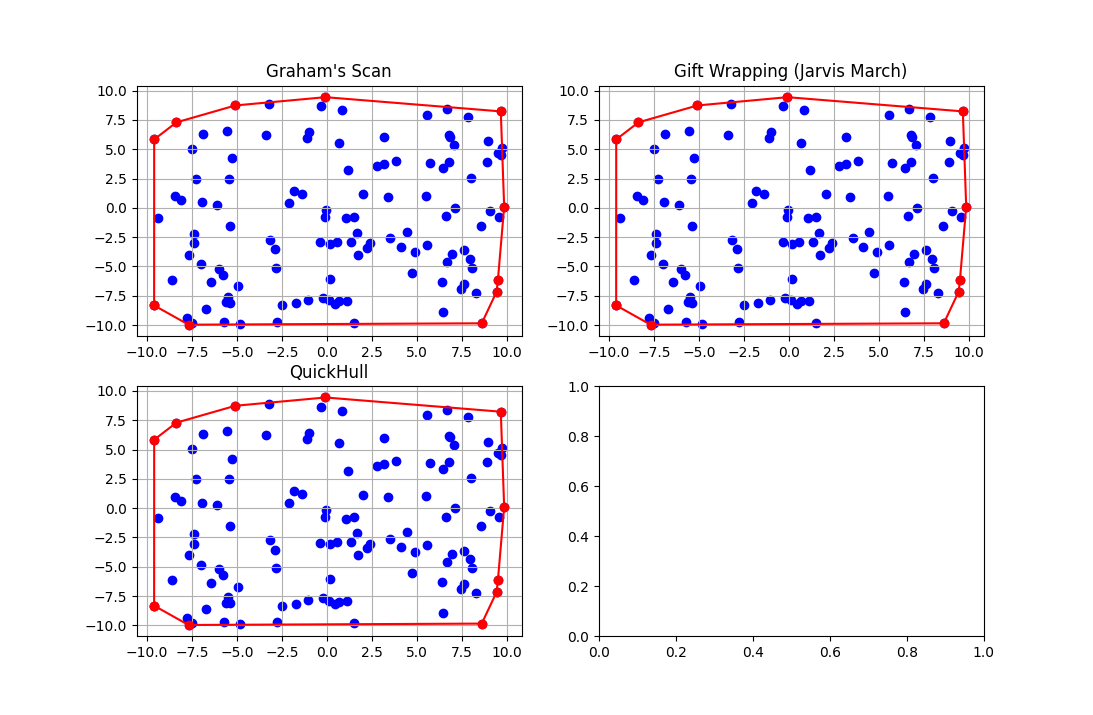
\includegraphics[width=0.7\linewidth]{Figure_1}
	\caption{Αποτέλεσμα Κυρτού Περιβλήματος για 120 τυχαία σημεία.}
	\label{fig:figure1}
\end{figure}

\subsection{Υπολογισμός Χρόνου Αλγορίθμων}

\begin{table}[ht]
	\centering
	\begin{tabular}{@{}lcc@{}}
		\toprule
		\textbf{Αλγόριθμος}            & \textbf{Χρόνος} \\ \midrule
		Graham's Scan                 & 0.000123                \\
		Gift Wrapping (Jarvis March)   & 0.000240                \\
		QuickHull                     & 0.000201                \\
		Divide and Conquer            & $\infty$                \\ \bottomrule
	\end{tabular}
	\caption{Comparison of Time Taken for Each Convex Hull Algorithm}
	\label{tab:convex-hull-times}
\end{table}

\section{Υλοποίηση Β: Γραμμικός Προγραμματισμός}

Οι περιορισμοί τις άσκησης εμφανίζονται γραφικά παρακάτω:

\begin{figure}[h!]
	\centering
	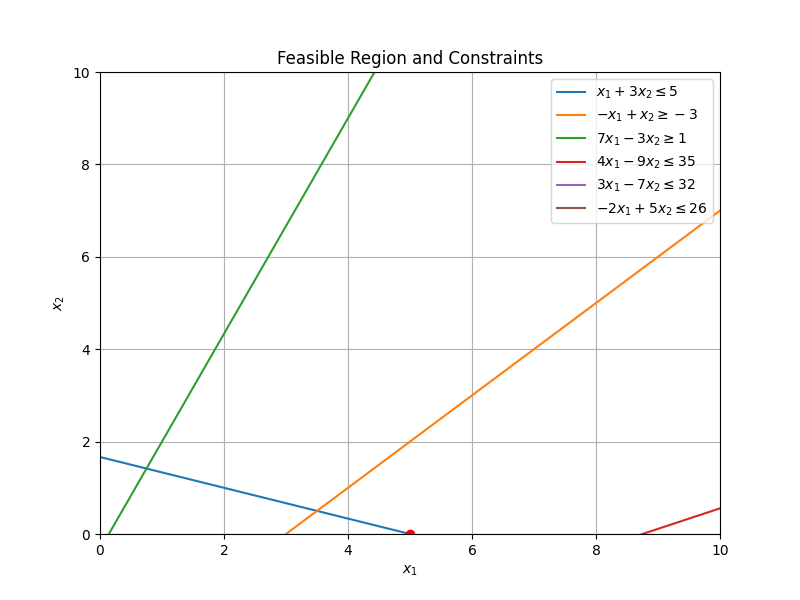
\includegraphics[width=0.7\linewidth]{Figure_2}
	\caption{Περιορισμοί και εφικτή περιοχή.}
	\label{fig:figure2}
\end{figure}

\section{Υλοποίηση Γ: Διάγραμμα Voronoi - Τριγωνοποίηση Delaunay}

Το διάγραμμα Voronoi εμφανίζεται παρακάτω:

\begin{figure}[h!]
	\centering
	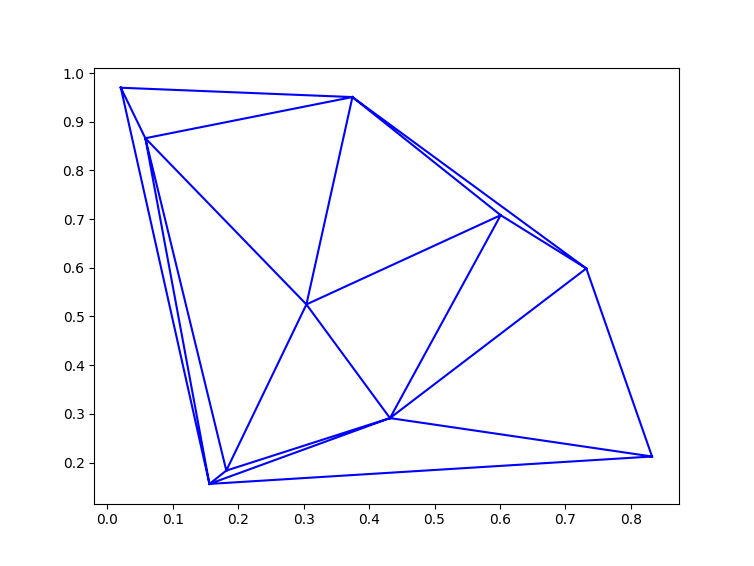
\includegraphics[width=0.7\linewidth]{Figure_3}
	\caption{Voronoi}
	\label{fig:figure3}
\end{figure}

Η αντιστοιχία Voronoi - Delaunay εμφανίζεται γραφικά παρακάτω:

\begin{figure}[h!]
	\centering
	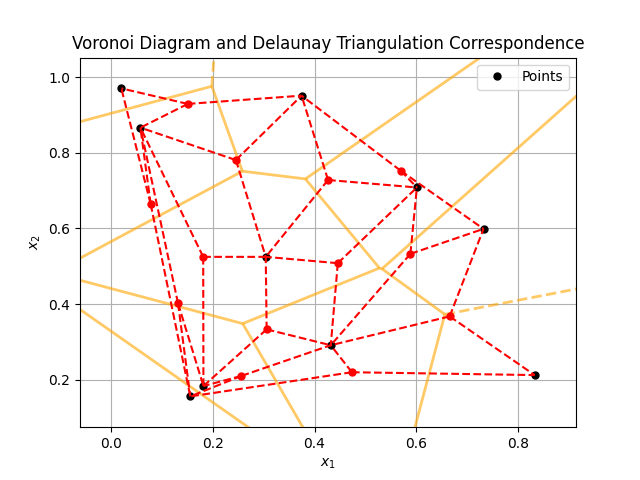
\includegraphics[width=0.7\linewidth]{Figure_4}
	\caption{Αντιστοιχία Voronoi - Delaunay}
	\label{fig:figure4}
\end{figure}

Η πολυπλοκότητα και των δύο αλγορίθμων είναι $\mathcal{O}(nlogn)$, το οποίο είναι ένδειξη χρήσης διαίρε και βασίλευε.
\newpage

\section{Υλοποίηση Δ: Γεωμετρική Αναζήτηση}

Το αποτέλεσμα εμφανίζεται σχηματικά παρακάτω:

\begin{figure}[h!]
	\centering
	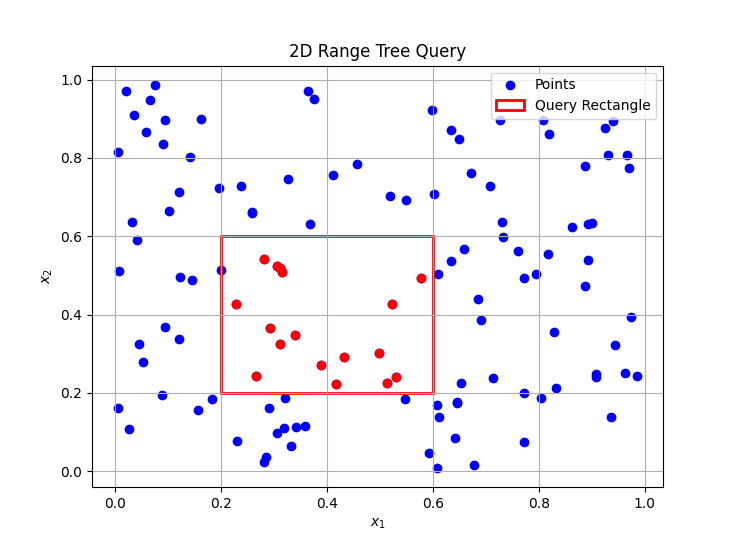
\includegraphics[width=0.7\linewidth]{Figure_5}
	\caption{Range tree με \textcolor{red}{ορθογώνια έκταση}.}
	\label{fig:figure5}
\end{figure}

Η λίστα των σημείων εντός της έκτασης παρουσιάζονται κατά την εκτέλεση του προγράμματος \verb|geom_search.py|.

\end{document}  